\documentclass[10pt]{article}
\usepackage[a4paper,margin=0.72in,headheight=21pt]{geometry}
\usepackage{mathptmx,graphicx,array,longtable,color,fancyhdr,url}
\def\UrlBreaks{\do\/\do\a\do\b\do\c\do\d\do\e\do\f\do\g\do\h\do\i\do\j\do\k\do\l\do\m\do\n\do\o\do\p\do\q\do\r\do\s\do\t\do\u\do\v\do\w\do\x\do\y\do\z\do\A\do\B\do\C\do\D\do\E\do\F\do\G\do\H\do\I\do\J\do\K\do\L\do\M\do\N\do\O\do\P\do\Q\do\R\do\S\do\T\do\U\do\V\do\W\do\X\do\Y\do\Z\do\0\do\1\do\2\do\3\do\4\do\5\do\6\do\7\do\8\do\9}
\definecolor{BorderBlue}{RGB}{38,91,145}\definecolor{PaleBlue}{RGB}{233,241,249}\definecolor{DarkInk}{RGB}{28,36,45}
\color{DarkInk}\setlength{\parindent}{0pt}\setlength{\parskip}{5pt}
\pagestyle{fancy}\fancyhf{}\lhead{DOC-2-096 R0--R4 negative-evidence arc}\rhead{Packaging-only backfill}\cfoot{\thepage}
\renewcommand{\headrulewidth}{0.8pt}\renewcommand{\headrule}{\hbox to\headwidth{\color{BorderBlue}\leaders\hrule height \headrulewidth\hfill}}
\newcommand{\boxnote}[1]{\noindent\fcolorbox{BorderBlue}{PaleBlue}{\parbox{0.94\linewidth}{#1}}}
\newcommand{\src}[1]{\par\vfill\noindent\parbox{\linewidth}{\raggedright\sloppy\scriptsize\color{BorderBlue}\textbf{Frozen source:} \texttt{#1}}}
\newcommand{\pg}[2]{\section*{#1}#2}
\begin{document}
\begin{center}\vspace*{1.2cm}{\Huge\color{BorderBlue}\textbf{Disease networks from bounded negative evidence: a five-round negative-result arc}}\\[8pt]{\Large DOC-2-096 / combined R0--R4 package}\\[16pt]{\large Submission-ready packaging-only backfill}\\[22pt]\fcolorbox{BorderBlue}{PaleBlue}{\parbox{0.82\linewidth}{\centering\textbf{Core conclusion.} Predictive triage is closed. What graduates is descriptive: bounded benign and conflicting evidence rewires ClinVar disease-network topology (R0), and simple evidence-burden rankings transport for database-activity review queues (R4) with no added model value. No calibrated predictor, clinical-risk, pathogenicity, or disease-severity claim is made.}}\\[28pt]\textbf{Frozen science date:} 21 September 2026\\\textbf{Package date:} 23 September 2026\\\textbf{Source repository commit:} 9b59730945b74a7059cf09ac5ae2aa5b2be634d4\end{center}
\vfill\textbf{Package contents.} Report and source; the complete frozen project tree (summary plus all five round trees: protocols, code, data, results, reports, reviews, provenance); one byte-identical reused figure and two deterministic figures; a read-only curator-queue exporter; golden and custody tests; provenance notes; a complete source-hash map with per-round maps; a manifest; and closeout records. Large raw ClinVar downloads remain external hash references and are not duplicated.\newpage

\pg{1. Abstract}{ClinVar benign and conflicting variant classifications are usually discarded as non-evidence. This project treated them as bounded network context and followed the consequence through five locked rounds. R0 built 581,228 stable-identifier gene-condition edges from a checksum-frozen live ClinVar snapshot and showed that high benign burden marks conflict-prone evidence neighborhoods (25.2 percentage-point higher conflict prevalence after exact stratification; direction replicated in four identifier-source strata) and that reliability weighting rewires 35.8\% of top-decile disease neighbors while preserving 80.4\% of high-review neighborhoods: a locked-gate success with a bounded claim. R1 stopped cleanly: the current submission snapshot cannot reconstruct historical assertion states without leakage, and it froze an ambiguity-aware condition crosswalk instead of a model. R2 obtained archived December 2020 and December 2023 snapshots, made the temporal test identifiable, and falsified transport: the R0 reliability score improved Brier by 4.50\% in development but was 0.16\% worse than raw counts in locked replication, with calibration slope 0.132 and negative controls losing only about 19\% of enrichment. R3 showed a frozen ranking ensemble did not beat simple conflict topology (replication top-decile 1.16x versus 2.60x; bootstrap interval 0.97--1.38 crossing 1) and exposed a risk-set orientation artifact. R4 separated competing risk sets; simple burden rankings transported for conflict emergence (2.22x), conflict resolution (2.69x), and review upgrade (2.37x), and no added model beat those baselines, so predictive triage closed by abstention under the locked rule.\par\boxnote{This package synthesizes frozen claims only. It introduces no recomputation, re-ranking, threshold change, cross-round statistic, or post hoc combined score. Each round's status is preserved separately.}}\src{frozen/PROJECT\_SUMMARY.md; frozen/rounds/*/*/report/FULL\_TECHNICAL\_REPORT.md}\newpage

\pg{2. Scope and non-claims}{This package combines the frozen R0--R4 artifacts of DOC-2-096 without rerunning, rescoring, filtering, or changing any science. It adds presentation, custody records, deterministic views of two frozen CSVs, a read-only exporter, and tests. R0's bounded positive is kept distinct from R1--R4's temporal, archive, ranking, and competing-risk limits; the arc is a coherent negative-evidence narrative, not a flattened positive one.\par\textbf{Non-claims.} No calibrated predictor of conflict or review outcomes. No clinical-risk, pathogenicity, disease-severity, or patient-triage claim. Benign evidence is context, never a gene-disease refutation. Queue outputs mean database-activity review priority only. R2's reliability ranking enrichment does not imply usable calibrated probabilities. R4's transporting simple burdens likely reflect ascertainment and testing volume.\par\textbf{Interpretation boundary.} A preserved failure is part of the result: R2, R3 and the R4 model gate are informative negatives with locked gates, reported with original populations, endpoints, denominators, thresholds, and caveats intact.}\src{frozen/PROJECT\_SUMMARY.md; frozen/rounds/*/*/README.md}\newpage

\pg{3. Locked sequence and methods chronology}{Every round locked its protocol before seeing its outcomes on 21 September 2026 (IST): R0 22:22, R1 22:32, R2 22:39, R3 22:44, R4 22:51. R0 audited a live checksum-frozen ClinVar snapshot (GRCh38) into gene-condition edges and tested the bounded negative-evidence claim under exact strata with negative controls. R1 attempted temporal transport from the same snapshot, proved it unidentifiable without leakage, and froze the condition crosswalk. R2 downloaded exact December 2020 and December 2023 archives, rebuilt each release's edges solely from its own tables, froze a 2020-only crosswalk, and ran the locked development (2020$\to$2023) and replication (2023$\to$current) evaluation. R3 reframed the failed predictor as ranking-only triage under a frozen ensemble and lost to the simplest baseline. R4 redesigned the targets as three competing risk sets and closed predictive triage when no added model beat simple burdens by the locked margin.\par\textbf{Protocol lock verification.} All seven locked-protocol sidecar hashes (R0 protocol.md and protocol.json, R1 protocol.md and protocol.json, R2/R3/R4 protocol.md) re-verify against the packaged bytes, as does the R1 crosswalk lock.}\src{frozen/rounds/*/*/protocol/LOCKED\_PROTOCOL.md; frozen/rounds/*/*/protocol/*.sha256}\newpage

\pg{4. R0 hypothesis and locked design}{Hypothesis: gene-condition edges supported only by pathogenic assertions differ topologically from edges whose submitted variants include both pathogenic and benign evidence, and contradiction burden identifies unstable evidence neighborhoods. The design preceded downloads and fixed stable identifiers (MedGen/OMIM/Orphanet), GRCh38, the positive threshold P$\ge$2, contradiction definitions (P$\ge$1 and B$\ge$1, or any conflicting-class variant), bounded benign burden B/(P+B) defined only where P+B$>$0, degree/review/source strata, projection weighting by reliability P/(P+B+conflicting+1), and success gates. A benign variant never deleted a positive edge and was never called a refutation.\par\textbf{Locked gate.} $\ge$10,000 stable-ID edges and $\ge$1,000 contradictory edges; burden associated with at least one prespecified instability endpoint after exact stratification; direction replicated in two source strata; reliability weighting changes $\ge$5\% of top-decile disease neighbors while preserving $\ge$80\% of high-review neighbors; negative controls smaller.}\src{frozen/rounds/DOC-2-096-R0-*/DOC-2-096-R0-negative-evidence/protocol/LOCKED\_PROTOCOL.md}\newpage

\pg{5. R0 results: locked-gate success, bounded claim}{The audit produced 581,228 stable-ID gene-condition edges over 21,608 genes and 31,819 conditions; 49,863 edges had P$\ge$2; 55,054 edges carried contradictory evidence and 40,683 positive edges were contradiction-bearing. Within positive edges, high benign burden was associated with a 25.2 percentage-point higher prevalence of conflicting-class variants after exact stratification by identifier source, gene degree, condition degree and review status (stratified risk difference 0.2522). The direction replicated in all four identifier-source strata (MONDO 0.277, MedGen 0.261, OMIM 0.237, Orphanet 0.233). Reliability weighting changed 35.8\% of top-decile disease neighbors across 368,470 projection pairs while preserving 80.4\% of neighbors built from high-review edges. The accession-initial negative-control dispersion (18.5 points) was smaller than the stratified instability effect. The high-benign-burden threshold was 0.557 among P+B evidence. All seven gate conditions passed.\par\boxnote{Bounded claim: benign evidence is useful network context, not absence of gene-disease association. Contradiction often marks allelic heterogeneity, phenotype granularity, mechanism specificity, or curation disagreement.}}\src{results/gate\_decision.json; results/source\_replication.csv; results/stratified\_instability.csv; report/FULL\_TECHNICAL\_REPORT.md (R0)}\newpage

\pg{6. R0 network figure}{\begin{center}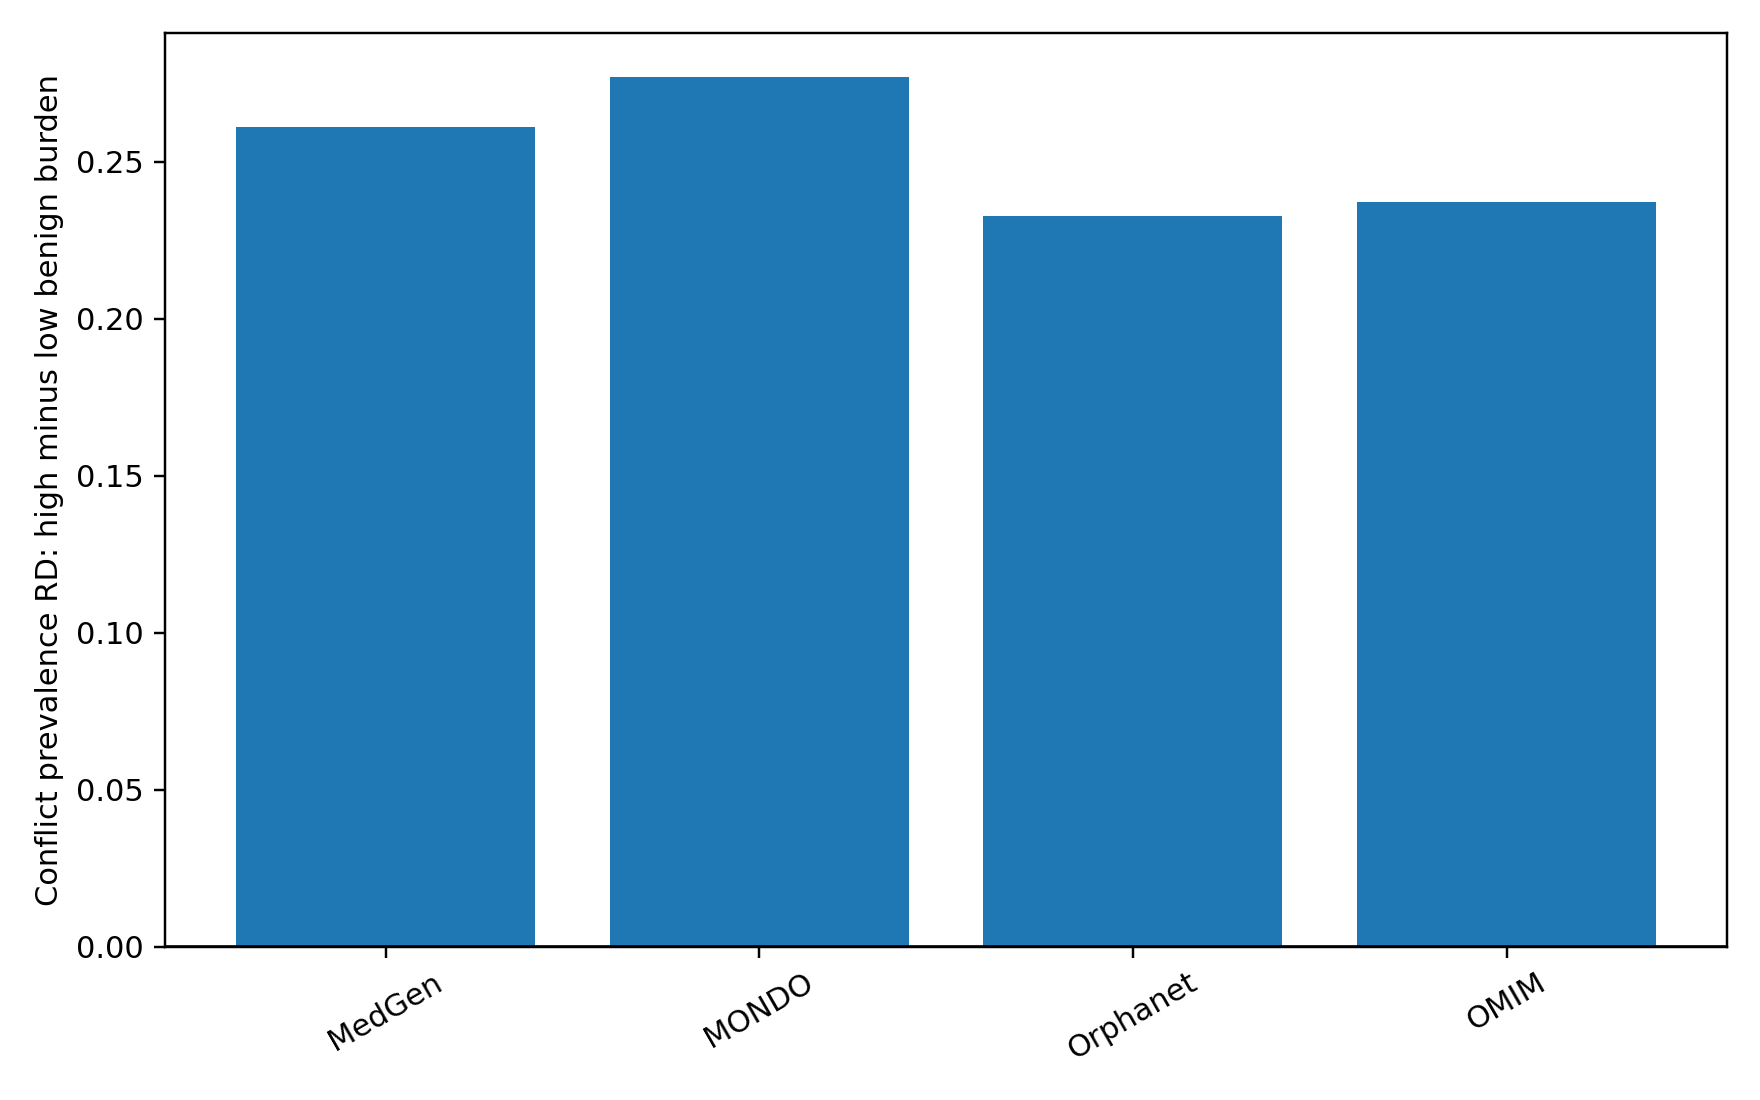
\includegraphics[width=0.86\linewidth]{../figures/r0_source_instability.png}\end{center}The frozen R0 figure shows the identifier-source replication of the stratified instability association. It is reused byte-identically from the frozen R0 tree; its SHA-256 is recorded in \texttt{figures/r0\_source\_instability.SOURCE.sha256} and it was not rerendered.}\src{figures/r0\_source\_instability.png; frozen R0 figures/source\_instability.png}\newpage

\pg{7. R1 hypothesis and temporal-identifiability stop}{Hypothesis: early negative-evidence topology predicts later conflict resolution and review upgrade. The locked design specified development through 2020, holdout 2021--2023, test $\ge$2024, SCV-base collapse, submitter clustering, calibration, and negative controls. The frozen audit then showed the design cannot be executed from the current snapshot: \texttt{submission\_summary} is a current snapshot of retained submissions with \texttt{DateLastEvaluated}; it lacks withdrawn and superseded states and past review status, so a 2020-cutoff development set would leak current retained assertions. No temporal model, AUROC, Brier score, or calibration claim was produced. The identifiability gate recorded \texttt{identifiability\_pass} set to \texttt{false} over 6,438,819 compressed snapshot lines.\par\boxnote{Status: CLEAN TEMPORAL-IDENTIFIABILITY STOP. This is an identifiability result, not a negative prediction result. Date permutation would not fix the leakage.}}\src{results/temporal\_identifiability.json; report/FULL\_TECHNICAL\_REPORT.md (R1)}\newpage

\pg{8. R1 condition crosswalk}{Before the stop, R1 froze a versioned ontology crosswalk built from identifier co-occurrence inside the same ClinVar phenotype slot, admitting a canonical component only when it contained at most one identifier per source. Result: 31,993 identifiers, 944 multi-source/single-source components, 54 ambiguous components retained unmapped, and 2,651 identifiers in unambiguous cross-source components. The low mapping yield is itself reported: most identifiers lack a unique cross-source co-occurrence in the current variant table. The crosswalk SHA-256 was locked (\texttt{2d068fee\ldots3ab}) and re-verifies against the packaged bytes. R1's preserved protocol specifies exactly how the temporal design should be executed unchanged against archived releases, which is what R2 then did.}\src{results/crosswalk\_audit.json; data/processed/condition\_crosswalk.csv; protocol/CROSSWALK\_LOCKED.sha256 (R1)}\newpage

\pg{9. R2 hypothesis and archive design}{Hypothesis: R0's reliability features transport prospectively across ClinVar release eras. Exact December 2020 and December 2023 variant and submission archives were downloaded, checksummed, and retained; the current snapshot came from R0's freeze. Each release's edges were built solely from its own variant table with no backfill of current IDs or review statuses. The ontology crosswalk was developed from 2020 only (24,565 identifiers, 255 ambiguous components); later unknown IDs stayed self-labeled. Cohorts: 30,990 baseline edges with 5,132 events (2020$\to$2023 development) and 49,548 edges with 6,062 events (2023$\to$current locked replication). Models (raw counts, positive-only, R0 reliability) were fit on development and applied unchanged to replication.\par\textbf{Locked gate.} Reliability must improve Brier $\ge$5\% over raw counts in both transitions, calibration slope 0.8--1.2, replication in two sources with leave-top-submitter-out survival, and both negative controls losing $\ge$50\% of enrichment.}\src{protocol/LOCKED\_PROTOCOL.md; report/FULL\_TECHNICAL\_REPORT.md (R2)}\newpage

\pg{10. R2 locked results: transport falsified}{\begin{center}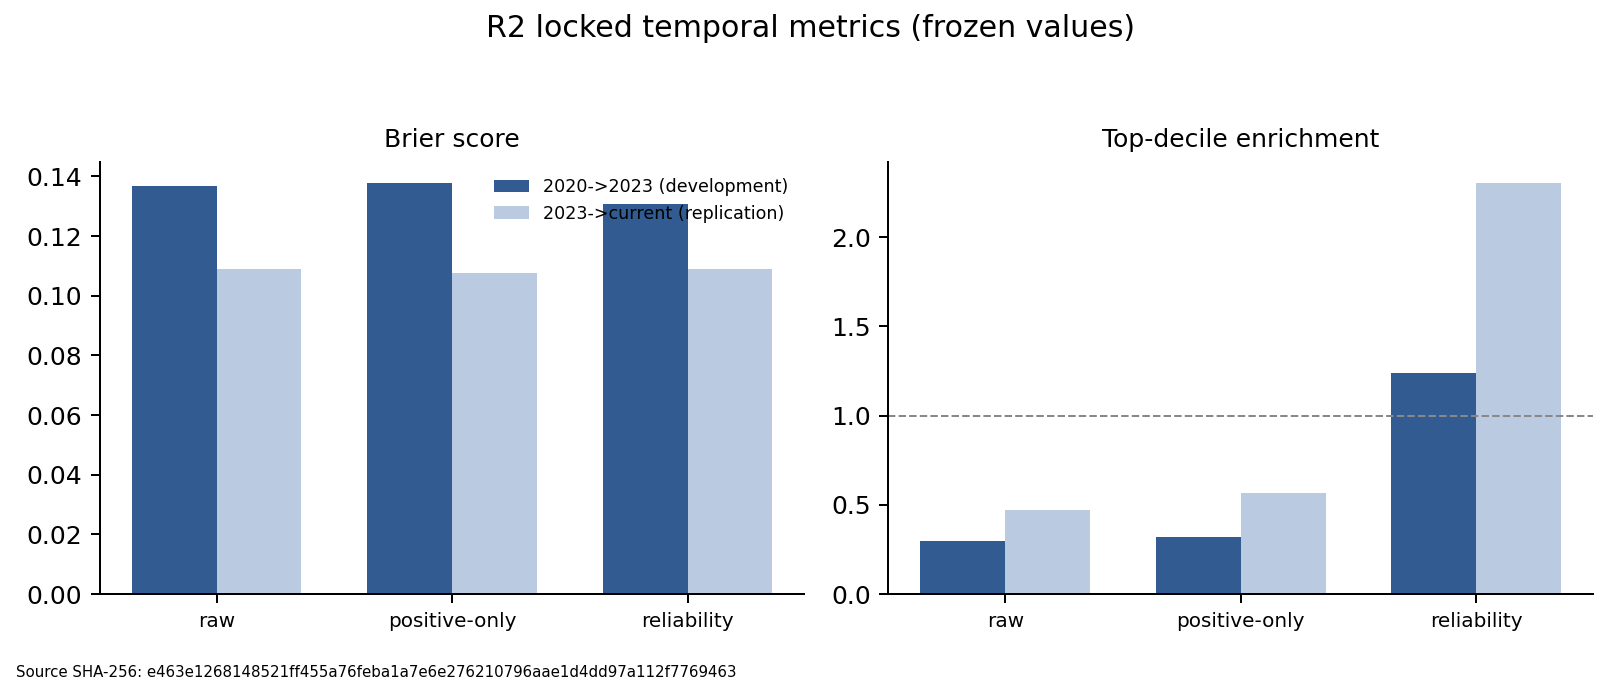
\includegraphics[width=0.98\linewidth]{../figures/r2_locked_transport.png}\end{center}\begin{tabular}{lrrrr}\hline Model&Dev Brier&Repl Brier&Repl slope&Repl top-decile\\\hline Raw counts&0.1369&0.1089&0.822&0.47x\\Positive-only&0.1379&0.1077&2.629&0.57x\\R0 reliability&0.1308&0.1090&0.132&2.30x\\\hline\end{tabular}\par The reliability model's 4.50\% development Brier improvement missed the 5\% gate; in locked replication it was 0.16\% worse than raw counts. Replication calibration slope 0.132 sits far outside 0.8--1.2. The figure renders only these frozen rows; its source hash is embedded and sidecar-recorded.}\src{results/gate\_decision.json; results/locked\_temporal\_metrics.csv; figures/r2\_locked\_transport.SOURCE.sha256}\newpage

\pg{11. R2 controls and interpretation}{Within-source label permutation and ontology-label randomization produced mean top-decile enrichment near 1.0 (1.0001, 1.0029), a loss of only about 19\% (0.191, 0.189) against the development reliability enrichment of 1.24x, not the required 50\%. The locked control gate failed alongside the Brier and calibration gates.\par\textbf{Interpretation preserved from the frozen report.} The striking combination of 2.30x ranking enrichment and poor Brier/calibration means the score can rank a volatile subset while its absolute probabilities do not transport; it must not be used as a calibrated decision threshold. ClinVar growth and curation changed between eras, so the meaning of an edge's benign/pathogenic ratio is not stationary. Reliability weighting remains useful for descriptive topology and possibly ranking, but not as an era-invariant calibrated predictor.\par\boxnote{Status: LOCKED-GATE FAILURE. Archived snapshots solved R1's identifiability problem and then falsified the transport claim: a true temporal negative, stronger than a random-split success.}}\src{results/negative\_controls.csv; results/gate\_decision.json; report/FULL\_TECHNICAL\_REPORT.md (R2)}\newpage

\pg{12. R3 hypothesis: ranking-only triage}{R3 separated ranking from the calibration that R2 had already failed. The only allowed product output was ``priority for evidence review,'' never a probability of pathogenicity, conflict, or clinical action. A development-frozen equal-rank ensemble of benign burden, conflict count, variant/testing burden, pathogenic count, benign count, and reliability was locked, with individual monotonic scores as comparators. The ranking gate required replication top-decile enrichment with a 95\% condition-block bootstrap interval above 1, at least 20\% improvement over the best simple baseline, direction in two ontology sources, and trajectory-block negative controls losing $\ge$50\% of enrichment. Ranking could pass while calibration failed; the two arms were kept distinct.}\src{protocol/LOCKED\_PROTOCOL.md; report/FULL\_TECHNICAL\_REPORT.md (R3)}\newpage

\pg{13. R3 results and the orientation artifact}{The frozen ensemble reached 1.27x top-decile enrichment in development but 1.16x in replication, with bootstrap interval 0.97--1.38 crossing 1. The best simple baseline, baseline conflict topology, reached 2.60x replication enrichment, so the ensemble lost decisively. At top 1\% and 5\%, replication enrichment was 0.90x; top-decile precision was 14.2\% against 12.2\% prevalence; NDCG 0.786 did not rescue weak top-k transport.\par\textbf{Mechanistic decomposition.} Development orientation was counterintuitive but reproducible: lower existing burden and higher reliability ranked later newly observed events, because edges already conflicting at baseline cannot experience conflict emergence. The simple baseline's strong score is tied to the same eligibility structure. This is target leakage by risk-set definition, not a deployable multifeature mechanism.\par\boxnote{Status: LOCKED RANKING GATE FAILURE. Calibration remains failed from R2. No graduation.}}\src{results/ranking.json; report/FULL\_TECHNICAL\_REPORT.md (R3)}\newpage

\pg{14. R4 hypothesis: competing risk sets}{R4 tested whether R3's artifact came from mixed risk sets. Three separate prospective targets were locked: conflict emergence (eligible only edges with no baseline conflict), conflict resolution (eligible only conflicted edges), and review upgrade (eligible only non-expert edges). Development 2020$\to$2023 froze score orientation; replication 2023$\to$current tested it. Scores were the simple burdens: raw variants, positive count, benign burden, reliability. The per-target ranking gate required $\ge$1,000 replication events, top-decile block-bootstrap interval above 1, $\ge$20\% over the best simple comparator, and direction agreement, with abstention below 1,000 events or under 2 absolute precision points. Predictive triage would close if all three failed. Output means review priority only.}\src{protocol/LOCKED\_PROTOCOL.md (R4)}\newpage

\pg{15. R4 results: transport without added model value}{\begin{center}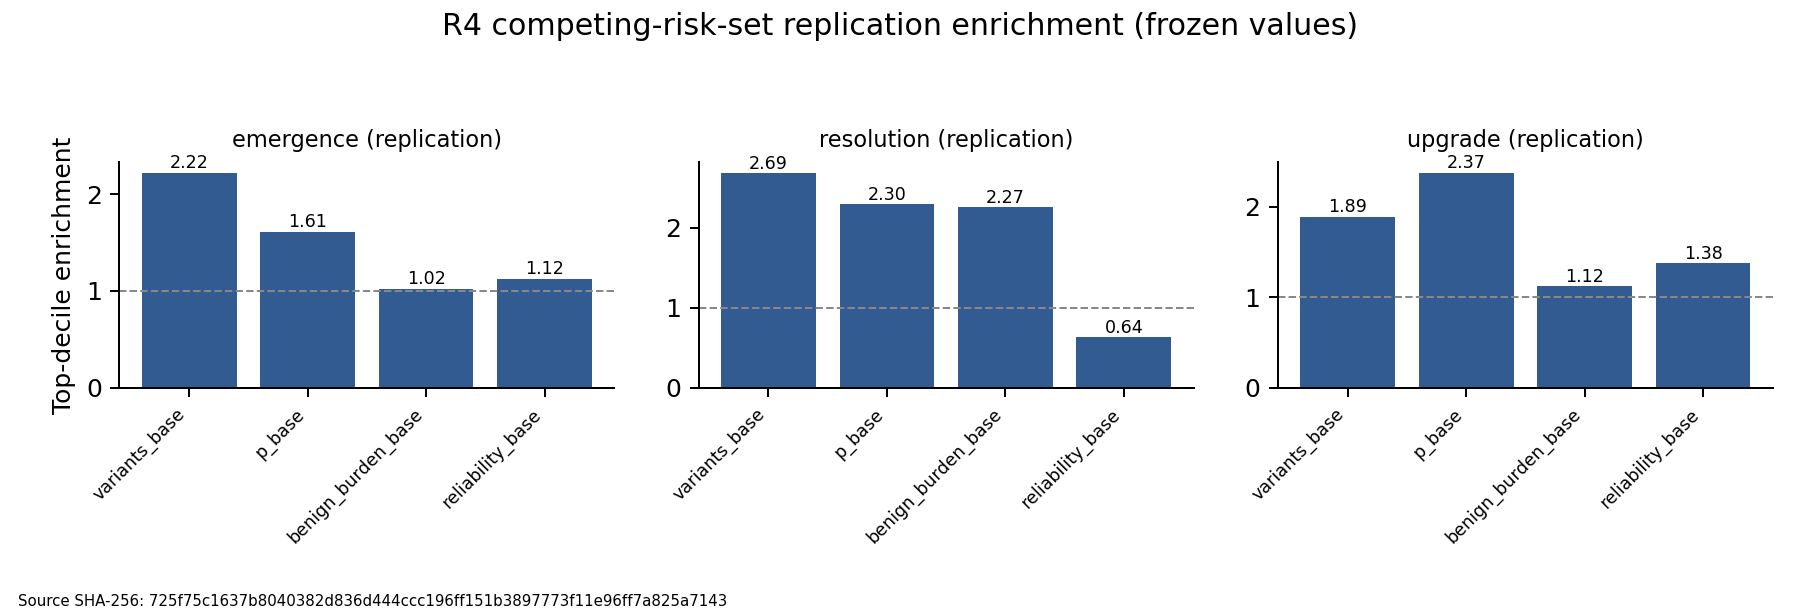
\includegraphics[width=0.98\linewidth]{../figures/r4_competing_risk_enrichment.png}\end{center}Separating risk sets fixed the eligibility artifact and revealed stable simple signals. Conflict emergence among clean edges: raw variant burden transported 2.02x$\to$2.22x, precision 67.2\% versus 30.3\% prevalence (4,671 replication events). Resolution among conflicted edges: lower variant burden transported 2.91x$\to$2.69x, precision 15.1\% versus 5.6\% (1,920 events). Review upgrade among non-expert edges: pathogenic count transported 1.68x$\to$2.37x, precision 7.36\% versus 3.10\% (1,467 events). The strongest scores were the simple baselines themselves; reliability and benign burden were consistently weaker or unstable, and no more complex frozen model had preregistered justification or evidence of incremental value. R4 abstained under the locked rule (0 of 3 targets passed) and closed predictive triage. The figure renders only frozen test-split rows.}\src{results/gate.json; results/competing\_risk\_metrics.csv; figures/r4\_competing\_risk\_enrichment.SOURCE.sha256}\newpage

\pg{16. Boundary synthesis: one negative-evidence arc}{The five rounds form a single coherent arc with each status intact. R0: benign and conflicting evidence, held as bounded context, measurably rewires disease-network topology (descriptive success). R1: current snapshots cannot support temporal claims without leakage (identifiability stop). R2: with real archives, reliability probabilities and calibration do not transport across eras, even though a volatile ranking signal exists (locked-gate failure). R3: a combined-outcome ranker fails uncertainty and baseline superiority, and its orientation artifact indicts the risk-set definition (ranking failure). R4: outcome-specific risk sets repair the artifact; simple evidence burdens transport, but no added model beats them, so the predictive product closes by abstention while the mechanism decomposition and the R0 descriptive topology stand.\par\boxnote{Graduated contribution: define the right risk set, prefer transparent evidence burden when it wins, and close the predictive model when it adds no value. The tool-shaped artifact is a read-only curator queue over frozen outputs, labeled database-activity priority, never clinical risk.}}\src{frozen/PROJECT\_SUMMARY.md; review/GRADUATION\_DECISION.md (R4)}\newpage

\pg{17. Claim-to-artifact map}{Every load-bearing claim in this report traces to a frozen artifact and SHA-256. Statuses are the frozen per-round labels, preserved separately.\par{\scriptsize\def\arraystretch{1.25}\begin{longtable}{p{0.32\linewidth}p{0.05\linewidth}p{0.26\linewidth}p{0.26\linewidth}}\hline \textbf{Claim}&\textbf{Round}&\textbf{Frozen artifact}&\textbf{SHA-256}\\\hline\endhead Benign burden marks conflict-prone neighborhoods: stratified risk difference 0.2522; replication in four source strata; network rewiring 35.8\% top-decile change with 80.4\% high-review preservation; gate passed&R0&results/gate\_decision.json&\url{08806eaebec8cf243bf9a94fcec6ce7620d62e9d2a54046e610e4162cc77a713}\\\hline Per-stratum risk differences behind the R0 association&R0&results/stratified\_instability.csv&\url{55bc01775aae976891e9bddebfc1618a6e9da849e6722b41e7ce9312cdb85080}\\\hline Four-stratum replication table (MONDO, MedGen, OMIM, Orphanet)&R0&results/source\_replication.csv&\url{5a61afb91988c1c2b246bf50ae16bb99326a94aa988b00301ef007ffbd4338d9}\\\hline Temporal prediction unidentifiable from current snapshot without leakage; identifiability\_pass=false&R1&results/temporal\_identifiability.json&\url{5402a459c44436d707ad3937657503ea6bead4aa0c53faaa0eb0810607ae7929}\\\hline Crosswalk yield: 31,993 identifiers, 944 components, 54 ambiguous, 2,651 mapped&R1&results/crosswalk\_audit.json&\url{6a01c2a31151bdb16b83232b3b4f57886bcbda4bde7bf8837b7fed10d2a1df99}\\\hline Frozen crosswalk bytes (lock re-verified)&R1&data/processed/condition\_crosswalk.csv&\url{2d068fee2bf4f56233e1c3bc18389dc42a4ea4bc75aac3cabab90ded02c2a3ab}\\\hline Transport falsified: Brier +4.50\% dev, $-$0.16\% repl; slope 0.132; controls lose $\sim$19\%; gate failed&R2&results/gate\_decision.json&\url{58f85a84842b429fe229e22d9a0c3955e913f5eb5e24ef932e1531fd1b8bb068}\\\hline Locked per-model transition metrics (Brier, slope, enrichment)&R2&results/locked\_temporal\_metrics.csv&\url{e463e1268148521ff455a76feba1a7e6e276210796aae1d4dd97a112f7769463}\\\hline Negative controls near 1.0 with 19\% loss&R2&results/negative\_controls.csv&\url{c569e4dfb59d5b5adbe50b2b2d3fbbd55996da0f79eafdc7a3708f57828ac2a2}\\\hline Ranking failure: replication 1.16x, CI 0.97--1.38, best simple 2.60x&R3&results/ranking.json&\url{64069ade2c675873153eb8cb198b9d4b02f457a8c18ee382c2800ac8b7b55e88}\\\hline Competing-risk transport and abstention: 2.22x/2.69x/2.37x; 0 targets passed; triage closed&R4&results/gate.json&\url{471e5d4c9a803a88483c878583a5101c5353ab718d6c87cc2af0581b69d6f67c}\\\hline Per-target, per-feature dev/test enrichment and precision&R4&results/competing\_risk\_metrics.csv&\url{725f75c1637b8040382d836d444ccc196ff151b3897773f11e96ff7a825a7143}\\\hline Graduation decision: no predictive-triage graduation; research finding graduates&R4&review/GRADUATION\_DECISION.md&\url{b1f0d75e6dcdbd3fad6c9b20e8f8e5cad7dffb2157971f19d97ef2d8f86c05eb}\\\hline\end{longtable}}}\src{provenance/SOURCE\_HASH\_MAP.tsv (full 87-item map)}\newpage

\pg{18. Limitations and honest negatives}{Aggregate ClinVar labels compress submitter histories; counts do not model allele frequency, molecular consequence, inheritance, or submitter dependence. Condition identifiers duplicate across MedGen, OMIM, Orphanet and MONDO, so source strata are not independent diseases. R2 used aggregate variant tables, not fully reconstructed SCV trajectories, and combined conflict-emergence with review-upgrade outcomes; submitter-blocked bootstrap and gene-size covariates remain incomplete. Condition self-labeling for post-2020 unknown IDs fragments some trajectories. R3 added no gene-size external covariates or full submitter-block resampling. R4's transporting burdens likely reflect ascertainment and testing volume and must not be read as disease biology. None of these gaps rescues a failed gate, and none is hidden: R2, R3, and the R4 model gate are reported as locked failures with their original denominators and thresholds.\par Conflicting evidence can reflect healthy scientific revision, not poor quality.}\src{frozen/rounds/*/*/report/FULL\_TECHNICAL\_REPORT.md; provenance/MISSING\_ARTIFACTS.md}\newpage

\pg{19. Reproducibility and environment}{Each frozen round carries its locked protocol with SHA-256 sidecar, executable analysis code, processed tables, result files, full technical report, internal review, source ledger, and a per-file manifest with bytes and SHA-256. All seven locked-protocol sidecars and the R1 crosswalk lock re-verify against the packaged bytes. Large raw ClinVar downloads (current snapshot; December 2020 and December 2023 archives) are external references: exact URLs, retrieval UTC, headers, and frozen SHA-256 values are recorded in the frozen provenance files and in \texttt{provenance/MISSING\_ARTIFACTS.md}; they are not duplicated. The sealed round tar bytes are not stored in the source repository; the extracted trees named by the tar hash prefixes are preserved byte-for-byte instead.\par The packaging environment needs only Python standard library (exporter, tests), matplotlib 3.10.9 (two deterministic figures), and pdfLaTeX (this report). Package verification never invokes the scientific pipeline.}\src{provenance/ENVIRONMENT.md; provenance/MISSING\_ARTIFACTS.md; frozen/rounds/*/*/provenance/file\_manifest\_sha256.csv}\newpage

\pg{20. Read-only curator-queue exporter}{The package includes \texttt{cli/curator\_queue\_export.py}, Python standard library only. It exposes the frozen outputs to a human curator: \texttt{verify}, \texttt{rounds}, \texttt{tables}, \texttt{summary}, \texttt{round-summary}, and \texttt{export}. Export selects by explicit round or exact frozen status label and emits stable sorted rows; every row carries source round, frozen claim status, source artifact path, source artifact SHA-256, and the original row identifier, with values as stored. It has no scoring, ranking, inference, cross-round merging, label change, threshold parameter, model call, network call, or write path.\par Golden tests compare canonical output byte-for-byte; a full export is run twice for determinism; a scope test requires refusal of a table outside a round; a corruption test flips one frozen digit in a temporary copy and requires verification to fail. The manifest check is bidirectional: listed hashes must match and unlisted extra bytes are rejected.}\src{cli/curator\_queue\_export.py; cli/README.md; tests/run\_tests.py; tests/golden/}\newpage

\pg{21. Provenance and custody}{Custody has three layers. First, \texttt{MANIFEST.sha256} hashes every regular package file except itself, with the archive hash as outer custody. Second, \texttt{provenance/SOURCE\_HASH\_MAP.tsv} maps all 87 copied frozen items back to the repository tree with per-file SHA-256 and MATCH status (87/87 MATCH, nonempty and complete), with per-round splits \texttt{SOURCE\_HASH\_MAP\_R0.tsv} through \texttt{R4}. Third, clean-restore evidence records verification from transferred archive bytes in a fresh directory: extraction, manifest check, exporter verification, tests, figure rerender, and PDF page count.\par The four custody defects found in the DOC-2-033 audit were preflighted here before submission: the source map is populated and complete; clean-restore evidence sits inside the archive and standalone beside it; every renderer and script needed for restore is transferred, including \texttt{figures/render\_figures.py}; and internal and outer custody metadata were regenerated from the final bytes and agree.\par Release requires the report, manifest, all irreplaceable bytes, and readback hashes to travel together. Repository commit and Drive upload are deliberately outside this package-creation step and await independent auditor approval.}\src{MANIFEST.sha256; provenance/SOURCE\_HASH\_MAP.tsv; closeout/CLEAN\_RESTORE\_EVIDENCE.txt; closeout/CLOSEOUT\_LEDGER.md}\newpage

\pg{22. Submission checklist and conclusion}{\begin{itemize}\item Combined R0--R4 report and source included; per-round statuses preserved separately.\item Core conclusion preserved: predictive triage closed; bounded descriptive topology and simple burden queues graduate.\item Frozen protocols, code, data, results, reports, reviews, and provenance included byte-for-byte for all five rounds.\item R0 figure reused byte-identically; two new figures trace to frozen CSV hashes and add no analysis.\item Read-only curator-queue exporter carries round, frozen status, source hash, and original identifier on every row; no scoring, ranking, merging, or label change.\item Golden, determinism, scope, corruption, extra-file, manifest, and restore checks recorded.\item Large raw downloads remain external hash references; nothing recreated from memory.\item Complete source-hash map, per-round maps, package manifest, and closeout ledger included.\end{itemize}\boxnote{Conclusion. DOC-2-096 is a disciplined negative-evidence arc: one bounded descriptive success, one identifiability stop, and three informative locked failures that together close predictive triage while delivering auditable database-activity review queues. Its value is the clearly drawn boundary, not a model.}}\src{PACKAGE\_MANIFEST.json; closeout/CLOSEOUT\_LEDGER.md}\end{document}
